\begin{center}
    \vspace*{1.5cm}
    {\fontsize{20}{20}\textbf{Bussvisor}}\\
    \vspace{0.7cm}
    {\fontsize{12}{12}\textit{Om Skånetrafiken själv får välja}}
\end{center}
\addtocwithheader{Bussvisor}  % Add entry to TOC and set header\noBackground
\noBackground

\newpage
\resetBackground


\subsubsection*{Hur man åker buss}
När en E:are åker buss ska den ha kul. Och kul har man bäst ihop med 
massa andra E:are och övriga Teknologer, förstås. Även busschauffören 
är det en fördel att vara på god fot med. Som alla vet älskar busschaufförer 
när deras passagerare sjunger högt, leker en massa och utför andra aktiviteter 
som lämnar ett bra intryck.
\\

När man åker buss verkar gravitationen och centripetalkrafter med 
mångdubblad styrka. När bussen svänger slungas passagerarna hejvilt 
runt i bussen! Detta är förstås tokroligt, så vid rondeller vill man 
så klart åka så många varv som möjligt för att få maximal utsöndring 
av endorfiner. För att övertyga busschauffören att även denne skulle 
tycka detta är en sanslöst bra idé, borde E:aren klappa och sjunga så 
högt det går; "Åh 2$\pi$ till, åh 2$\pi$ till, åh 2$\pi$ till..."
\\

Man kan även utsättas för diverse faror längs vägen! När broar 
och viadukter så där lömskt dyker upp är det livsviktigt att ducka 
för att inte slå i huvudet. Likaså när bussen åker över en bro eller 
viadukt måste man hoppa så att inte bussen tyngs ned alltför mycket 
och därmed saboterar bron. Träning är förstås viktigt och man kan 
aldrig riktigt veta vad som finns utanför. Det är lika bra att hålla 
andan så länge man är i en.
\\

Lycka till med Öresundsbron, gott folk!

\newpage

\subsection*{Bussången} 
\index[alfa]{Bussången}
\index[anfa]{Förr när man skulle bort}
\songinfo{Mel: Jag är en astronaut\\
Sjunges på bred skånska}

\begin{parse lines}[\noindent]{#1\\}
    Förr när man skulle bort
    lång väg såväl som kort
    fick man ta cykeln eller gå
    nu är det inte så

    Fööör...
    Nu kan vi åka buss
    förar'n bestämmer kurs
    Fönstren är många, ratten rund
    här i vår buss från Lund

    Nu ska vi leka bin
    här i vår busskabin
    Buzz, buzz, buzz, buzz, 
    buzz, buzz, buzz, buzz,
    buzz, buzz, buzz, åka buss!
\end{parse lines}

\vissteduatt{Visste du att E-styret 2002 åkte 400 varv i en rondell för att fira\\E-sektionens 40 års jubileum?}

\newpage


\subsection*{Busschaufförsvisan} 
\index[alfa]{Busschaufförsvisan}
\index[anfa]{Att vara elektriker är inte roligt}
\songinfo{Mel: Temperaturen\\
Ur Lundaspexet Biggles i öknen 1989}

\begin{parse lines}[\noindent]{#1\\}
    Att vara elektriker är inte roligt,
    köra en buss är just det som jag vill
    Att växla och tuta och blinka till höger
    Jubel i busskön när jag stannar till

    För ettan och tvåan och trean och fyran
    Ettan och tvåan och trean och broms! 
    Ettan och tvåan och trean och fyran,
    ettan och tvåan och trean och STOPP!

    Unga ska stå upp så gamla får sitta,
    fast ej på min stol för den är ju min
    Drar du i snöret så stannar jag gärna
    GÅ BAK I BUSSEN! så kommer fler in

    För ettan och tvåan och trean och fyran
    Ettan och tvåan och trean och broms! 
    Ettan och tvåan och trean och fyran,
    ettan och tvåan och trean och STOPP!
\end{parse lines}

\vissteduatt{Visste du att E-styret 2012 åkte 500 varv i en rondell för att fira\\E-sektionens 50 års jubileum?}

\newpage

\subsection*{Den bereste studentens visa} 
\index[alfa]{Den bereste studentens visa}
\index[anfa]{Jag har smakat drycker ifrån jordens alla vrår}
\songinfo{Mel: Man ska ha husvagn}

\begin{parse lines}[\noindent]{#1\\}
    Jag har smakat drycker ifrån jordens alla vrår
    Smuttat irländsk whiskey och i Aalborg ta'tt en tår
    Ouze ifrån Grekland, druckit saké med japan
    Tequila-race det har jag kört med äkta mexikan

    Jag far till Tyskland, där kan man köpa öl och sekt
    Till Vatikanen, får nattvardsvin för min kollekt
    Jag dricker vodka när ryska vädret blir för kallt
    Ja, jag har rest och druckit överallt

    På Kuba har jag druckit rom, i Rom jag druckit grappa
    Sliskigt söta drinkar på en bar i Aya Napa
    I Frankrike jag har testat varje druva från Bordeaux
    I Spanien jag sänker en Sangria eller två

    Jag far till Polen, och slipper undan våran skatt
    Med båt till Danmark, och köper sprit med mängdrabatt
    Och sen på Mallis, jag får enorm promillehalt
    Ja, jag har rest och druckit överallt

    Heroin från Amsterdam och Arrak från Sri Lanka 
    I Finland bränns det mesta själv men träsprit smakar planka
    I USA jag släpper loss med Coke och Rohypnol
    I Dublin med en Guinness-öl jag utbringar en skål

\end{parse lines}

\vissteduatt{Visste du att E-styret 2022 åkte 600 varv för att fira\\E-sektionens 60 års jubileum?}

\newpage
\noBackground

\begin{textblock*}{3cm}(5.8cm,6.3cm) % {width}(x, y)
    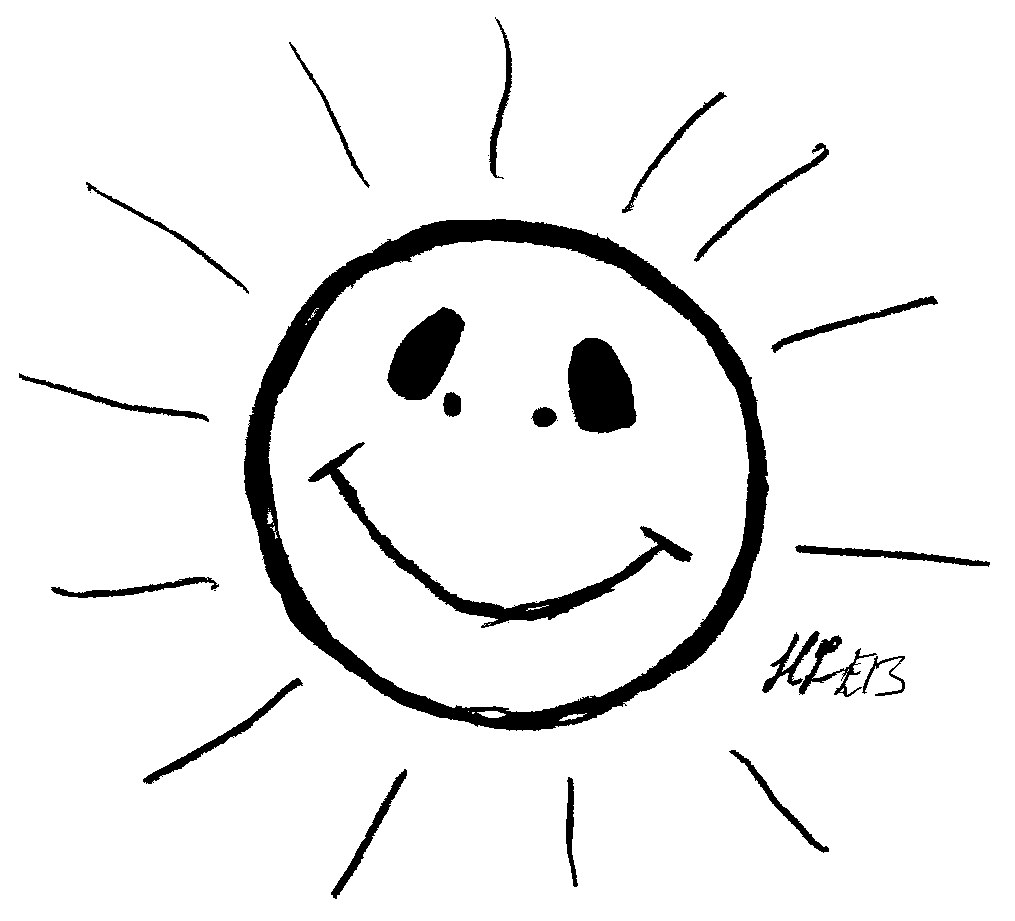
\includegraphics[width=4.3cm]{./bilder/sol.png}
\end{textblock*}

\begin{parse lines}[\noindent]{#1\\}

    Fast här i Lund, så är man jämt i glädjens hus
    Ja, här i Lund, så kan man få ett billigt rus
    Ja, här i Lund, så får man dricka vad man vill
    Så säg Gutår och drick varandra till - Skål!
\end{parse lines}

\vspace*{0.5 cm}
\subsection*{25 grader och sol i Helsingborg} 
\index[alfa]{25 grader och sol i Helsingborg}
\index[anfa]{Det är 25 grader och sol i Helsingborg}
\songinfo{Mel: She'll Be Coming 'Round the Mountain}

\begin{parse lines}[\noindent]{#1\\}
    ||: Det är 25 grader och sol i Helsingborg :||
    ||: Det är 25 grader och sol :||
    Det är 25 grader och sol i Helsingborg
\end{parse lines}

\vspace*{0.5 cm}
\subsection*{En busschaufför} 
\index[alfa]{En busschaufför}
\index[anfa]{En busschaufför}
\songinfo{Mel: O Tannenbaum}

\begin{parse lines}[\noindent]{#1\\}
    En busschaufför, en busschaufför,
    det är en man med glatt humör
    Och har han inget glatt humör,
    så är han ingen busschaufför
    En busschaufför, en busschaufför,
    det är en man med glatt humör
\end{parse lines}

\vissteduatt{Visste du att i baren får man dricka vad man vill?}

\newpage
\resetBackground

\subsection*{Morbid busslåt} 
\index[alfa]{Morbid busslåt}
\index[anfa]{Morbid busslåt}
\songinfo{Mel: Båtlåt}

\begin{parse lines}[\noindent]{#1\\}
    Det var en buss som sa till en annan:
    - Vad du var stilig, din lack är alldeles för grann
    Vi prejas lite grann och repar ner varann
    Som bara bussar kan

    Badda bam bam bam bam
    Badda bam bam bam

    Andra bussen sa: - Klart att jag vill va'
    med och krocka, krossa din stiliga för
    Vi varann förstör, busschauffören dör
    Av vägen sen vi kör
    Badda bam bam bam bam
    Badda bam bam bam

    Sedan kan vi slå en och kanske två
    våldsamma volter, landa nånstans vid en bäck
    Rulla lite däck, bensintanken är läck
    Och elden är ej släckt
    Badda bam bam bam bam
    Badda bam bam BOOM!
\end{parse lines}

\vissteduattlong{Visste du att Tandem var tvungen att ändra sina  regler kring växling\\av cyklare eftersom E-sektionen en gång i tiden var för snabba och\\cyklade ifrån alla?}

\newpage

\subsection*{Udflykt till Danmark} 
\index[alfa]{Udflykt till Danmark}
\index[anfa]{Om du har det trist i Lund, åk över Öresund}
\songinfo{Mel: Mitt lilla fejs och jag\\
K-sektionen Sångarstriden 1992}

\begin{parse lines}[\noindent]{#1\\}
    Om du har det trist i Lund, åk över Öresund
    Sätt dig på en färja, se'n så kan du härja
    Köp en öl, köp en till eller Köpenhamn
    köp så mycket öl du vill, smuggla om du kan

    Man kan se på konst, jovisst, på Louisiana
    men visst är det ganska trist, bara gå och glana
    Så vi kör till Helsingör, köper lite smör
    Heja Danmark friskt humör, sjunger vi i kör

    Många søde piger finns, dejligt sensuella
    men man bör se upp med kvinns, tänk på salmonella
    Lajbans hela natten lång, festa som en vilde
    Rockmusik och hålligång, värre än Roskilde

    Nästa morgon, nästan död, står man där i tullen
    Näsan lyser vit och röd, halsen den är svullen
    Jag ska smuggla kött och öl, men vad smugglar du?
    Och du svarar med ett bröl: "Den lille havefrue!"
\end{parse lines}

\vissteduatt{Visste du att i Linköping finns Sveriges största rondell,\\
Vallarondellen?}

\newpage
